\documentclass[twoside]{book}

% Packages required by doxygen
\usepackage{fixltx2e}
\usepackage{calc}
\usepackage{doxygen}
\usepackage[export]{adjustbox} % also loads graphicx
\usepackage{graphicx}
\usepackage[utf8]{inputenc}
\usepackage{makeidx}
\usepackage{multicol}
\usepackage{multirow}
\PassOptionsToPackage{warn}{textcomp}
\usepackage{textcomp}
\usepackage[nointegrals]{wasysym}
\usepackage[table]{xcolor}

% Font selection
\usepackage[T1]{fontenc}
\usepackage[scaled=.90]{helvet}
\usepackage{courier}
\usepackage{amssymb}
\usepackage{sectsty}
\renewcommand{\familydefault}{\sfdefault}
\allsectionsfont{%
  \fontseries{bc}\selectfont%
  \color{darkgray}%
}
\renewcommand{\DoxyLabelFont}{%
  \fontseries{bc}\selectfont%
  \color{darkgray}%
}
\newcommand{\+}{\discretionary{\mbox{\scriptsize$\hookleftarrow$}}{}{}}

% Page & text layout
\usepackage{geometry}
\geometry{%
  a4paper,%
  top=2.5cm,%
  bottom=2.5cm,%
  left=2.5cm,%
  right=2.5cm%
}
\tolerance=750
\hfuzz=15pt
\hbadness=750
\setlength{\emergencystretch}{15pt}
\setlength{\parindent}{0cm}
\setlength{\parskip}{3ex plus 2ex minus 2ex}
\makeatletter
\renewcommand{\paragraph}{%
  \@startsection{paragraph}{4}{0ex}{-1.0ex}{1.0ex}{%
    \normalfont\normalsize\bfseries\SS@parafont%
  }%
}
\renewcommand{\subparagraph}{%
  \@startsection{subparagraph}{5}{0ex}{-1.0ex}{1.0ex}{%
    \normalfont\normalsize\bfseries\SS@subparafont%
  }%
}
\makeatother

% Headers & footers
\usepackage{fancyhdr}
\pagestyle{fancyplain}
\fancyhead[LE]{\fancyplain{}{\bfseries\thepage}}
\fancyhead[CE]{\fancyplain{}{}}
\fancyhead[RE]{\fancyplain{}{\bfseries\leftmark}}
\fancyhead[LO]{\fancyplain{}{\bfseries\rightmark}}
\fancyhead[CO]{\fancyplain{}{}}
\fancyhead[RO]{\fancyplain{}{\bfseries\thepage}}
\fancyfoot[LE]{\fancyplain{}{}}
\fancyfoot[CE]{\fancyplain{}{}}
\fancyfoot[RE]{\fancyplain{}{\bfseries\scriptsize Generated by Doxygen }}
\fancyfoot[LO]{\fancyplain{}{\bfseries\scriptsize Generated by Doxygen }}
\fancyfoot[CO]{\fancyplain{}{}}
\fancyfoot[RO]{\fancyplain{}{}}
\renewcommand{\footrulewidth}{0.4pt}
\renewcommand{\chaptermark}[1]{%
  \markboth{#1}{}%
}
\renewcommand{\sectionmark}[1]{%
  \markright{\thesection\ #1}%
}

% Indices & bibliography
\usepackage{natbib}
\usepackage[titles]{tocloft}
\setcounter{tocdepth}{3}
\setcounter{secnumdepth}{5}
\makeindex

% Hyperlinks (required, but should be loaded last)
\usepackage{ifpdf}
\ifpdf
  \usepackage[pdftex,pagebackref=true]{hyperref}
\else
  \usepackage[ps2pdf,pagebackref=true]{hyperref}
\fi
\hypersetup{%
  colorlinks=true,%
  linkcolor=blue,%
  citecolor=blue,%
  unicode%
}

% Custom commands
\newcommand{\clearemptydoublepage}{%
  \newpage{\pagestyle{empty}\cleardoublepage}%
}

\usepackage{caption}
\captionsetup{labelsep=space,justification=centering,font={bf},singlelinecheck=off,skip=4pt,position=top}

%===== C O N T E N T S =====

\begin{document}

% Titlepage & ToC
\hypersetup{pageanchor=false,
             bookmarksnumbered=true,
             pdfencoding=unicode
            }
\pagenumbering{roman}
\begin{titlepage}
\vspace*{7cm}
\begin{center}%
{\Large My Project }\\
\vspace*{1cm}
{\large Generated by Doxygen 1.8.11}\\
\end{center}
\end{titlepage}
\clearemptydoublepage
\tableofcontents
\clearemptydoublepage
\pagenumbering{arabic}
\hypersetup{pageanchor=true}

%--- Begin generated contents ---
\chapter{To Compile Program}
\label{md_README}
\hypertarget{md_README}{}
{\ttfamily javac \hyperlink{_chord_8java}{Chord.\+java} \hyperlink{_chord_user_8java}{Chord\+User.\+java} \hyperlink{_file_stream_8java}{File\+Stream.\+java}} \subsection*{To run Program}

{\ttfamily java \hyperlink{class_chord_user}{Chord\+User} $<$port\+\_\+number$>$} for example java \hyperlink{class_chord_user}{Chord\+User} 3000 
\chapter{Hierarchical Index}
\section{Class Hierarchy}
This inheritance list is sorted roughly, but not completely, alphabetically\+:\begin{DoxyCompactList}
\item \contentsline{section}{Chord\+User}{\pageref{class_chord_user}}{}
\item Input\+Stream\begin{DoxyCompactList}
\item \contentsline{section}{File\+Stream}{\pageref{class_file_stream}}{}
\end{DoxyCompactList}
\item Remote\begin{DoxyCompactList}
\item \contentsline{section}{Chord\+Message\+Interface}{\pageref{interface_chord_message_interface}}{}
\begin{DoxyCompactList}
\item \contentsline{section}{Chord}{\pageref{class_chord}}{}
\end{DoxyCompactList}
\end{DoxyCompactList}
\item Serializable\begin{DoxyCompactList}
\item \contentsline{section}{File\+Stream}{\pageref{class_file_stream}}{}
\end{DoxyCompactList}
\item Unicast\+Remote\+Object\begin{DoxyCompactList}
\item \contentsline{section}{Chord}{\pageref{class_chord}}{}
\end{DoxyCompactList}
\end{DoxyCompactList}

\chapter{Class Index}
\section{Class List}
Here are the classes, structs, unions and interfaces with brief descriptions\+:\begin{DoxyCompactList}
\item\contentsline{section}{\hyperlink{class_chord}{Chord} }{\pageref{class_chord}}{}
\item\contentsline{section}{\hyperlink{interface_chord_message_interface}{Chord\+Message\+Interface} }{\pageref{interface_chord_message_interface}}{}
\item\contentsline{section}{\hyperlink{class_chord_user}{Chord\+User} }{\pageref{class_chord_user}}{}
\item\contentsline{section}{\hyperlink{class_file_stream}{File\+Stream} }{\pageref{class_file_stream}}{}
\end{DoxyCompactList}

\chapter{File Index}
\section{File List}
Here is a list of all files with brief descriptions\+:\begin{DoxyCompactList}
\item\contentsline{section}{C\+E\+C\+S327/assignment1/\hyperlink{ftpclient_8cpp}{ftpclient.\+cpp} }{\pageref{ftpclient_8cpp}}{}
\end{DoxyCompactList}

\chapter{Class Documentation}
\hypertarget{class_chord}{}\section{Chord Class Reference}
\label{class_chord}\index{Chord@{Chord}}
Inheritance diagram for Chord\+:\begin{figure}[H]
\begin{center}
\leavevmode
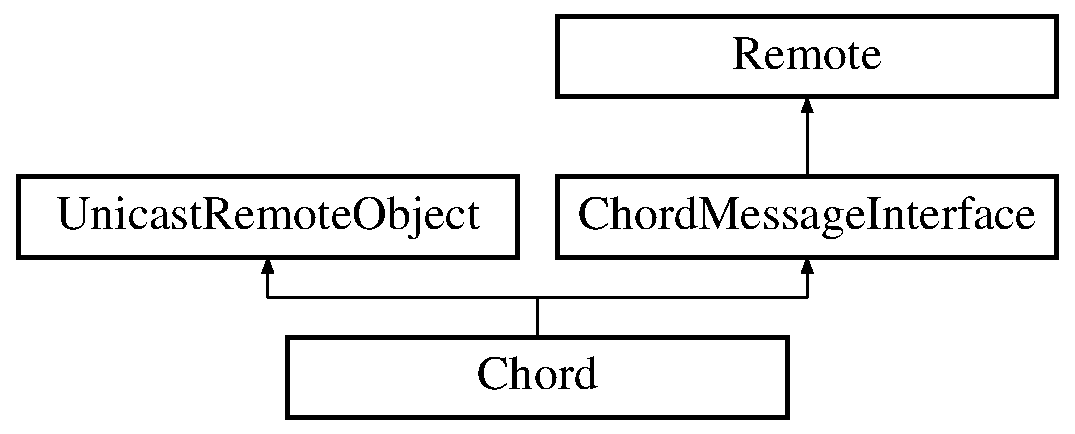
\includegraphics[height=3.000000cm]{class_chord}
\end{center}
\end{figure}
\subsection*{Public Member Functions}
\begin{DoxyCompactItemize}
\item 
\hyperlink{interface_chord_message_interface}{Chord\+Message\+Interface} \hyperlink{class_chord_a2fd46745a549fb8447f2cb7e32e8b07b}{rmi\+Chord} (String ip, int port)
\item 
Boolean \hyperlink{class_chord_ad88edc3a01395c31dd0ae209195a2e08}{is\+Key\+In\+Semi\+Close\+Interval} (int key, int key1, int key2)
\item 
Boolean \hyperlink{class_chord_a711a8c4e621940da4c48c1ba60479bd7}{is\+Key\+In\+Open\+Interval} (int key, int key1, int key2)
\item 
void \hyperlink{class_chord_a1133387e1312ead8daf5c94c11ff3b78}{put} (int guid, Input\+Stream stream)  throws Remote\+Exception
\begin{DoxyCompactList}\small\item\em Stores the file for given guid. \end{DoxyCompactList}\item 
Input\+Stream \hyperlink{class_chord_a6fa6e161d33e337f53cc0f3e38e1791b}{get} (int guid)  throws Remote\+Exception 
\begin{DoxyCompactList}\small\item\em returns the file of a given guid \end{DoxyCompactList}\item 
void \hyperlink{class_chord_ab16ffb81226d722399a46d1acfd70e60}{delete} (int guid)  throws Remote\+Exception 
\begin{DoxyCompactList}\small\item\em Fires after file has been found. \end{DoxyCompactList}\item 
int \hyperlink{class_chord_a7c6a50aff653bafc040f923c93061bdb}{get\+Id} ()  throws Remote\+Exception 
\item 
boolean \hyperlink{class_chord_a0a677ced19cc0cb5afd2a695977aeb95}{is\+Alive} ()  throws Remote\+Exception 
\item 
\hyperlink{interface_chord_message_interface}{Chord\+Message\+Interface} \hyperlink{class_chord_a3f1aadce3820e808c80662bb61a58e34}{get\+Predecessor} ()  throws Remote\+Exception
\item 
\hyperlink{interface_chord_message_interface}{Chord\+Message\+Interface} \hyperlink{class_chord_aa53f4f7c97122395a33d064460538db0}{locate\+Successor} (int key)  throws Remote\+Exception
\item 
\hyperlink{interface_chord_message_interface}{Chord\+Message\+Interface} \hyperlink{class_chord_a77a9443c945cf5482f59edf685c1dc70}{closest\+Preceding\+Node} (int key)  throws Remote\+Exception 
\item 
void \hyperlink{class_chord_ace0b8d2768590d7527af155c6573cae7}{join\+Ring} (String ip, int port)  throws Remote\+Exception 
\item 
void \hyperlink{class_chord_a65c855dc1d8c6a82545899cb823dba2e}{finding\+Next\+Successor} ()
\item 
void \hyperlink{class_chord_a8a4b7a1cd88cb3f607ada0629f2ff2dd}{stabilize} ()
\item 
void \hyperlink{class_chord_a4de8b8464782dd96d88deeb35b2f27a2}{notify} (\hyperlink{interface_chord_message_interface}{Chord\+Message\+Interface} j)  throws Remote\+Exception 
\item 
void \hyperlink{class_chord_a02763f74bbd986baa7e6567bf9dc3c95}{fix\+Fingers} ()
\item 
void \hyperlink{class_chord_a530b2ab58c9f4026dadf4293c38c4450}{check\+Predecessor} ()
\item 
\hyperlink{class_chord_aed079e86ebb63da4af055ca324a74274}{Chord} (int port)  throws Remote\+Exception 
\end{DoxyCompactItemize}
\subsection*{Static Public Attributes}
\begin{DoxyCompactItemize}
\item 
static final int \hyperlink{class_chord_a864e0b4011dc157c78a06dd951c6d9ac}{M} = 2
\end{DoxyCompactItemize}


\subsection{Constructor \& Destructor Documentation}
\index{Chord@{Chord}!Chord@{Chord}}
\index{Chord@{Chord}!Chord@{Chord}}
\subsubsection[{\texorpdfstring{Chord(int port)}{Chord(int port)}}]{\setlength{\rightskip}{0pt plus 5cm}Chord.\+Chord (
\begin{DoxyParamCaption}
\item[{int}]{port}
\end{DoxyParamCaption}
) throws Remote\+Exception}\hypertarget{class_chord_aed079e86ebb63da4af055ca324a74274}{}\label{class_chord_aed079e86ebb63da4af055ca324a74274}


\subsection{Member Function Documentation}
\index{Chord@{Chord}!check\+Predecessor@{check\+Predecessor}}
\index{check\+Predecessor@{check\+Predecessor}!Chord@{Chord}}
\subsubsection[{\texorpdfstring{check\+Predecessor()}{checkPredecessor()}}]{\setlength{\rightskip}{0pt plus 5cm}void Chord.\+check\+Predecessor (
\begin{DoxyParamCaption}
{}
\end{DoxyParamCaption}
)}\hypertarget{class_chord_a530b2ab58c9f4026dadf4293c38c4450}{}\label{class_chord_a530b2ab58c9f4026dadf4293c38c4450}
\index{Chord@{Chord}!closest\+Preceding\+Node@{closest\+Preceding\+Node}}
\index{closest\+Preceding\+Node@{closest\+Preceding\+Node}!Chord@{Chord}}
\subsubsection[{\texorpdfstring{closest\+Preceding\+Node(int key)}{closestPrecedingNode(int key)}}]{\setlength{\rightskip}{0pt plus 5cm}{\bf Chord\+Message\+Interface} Chord.\+closest\+Preceding\+Node (
\begin{DoxyParamCaption}
\item[{int}]{key}
\end{DoxyParamCaption}
) throws Remote\+Exception}\hypertarget{class_chord_a77a9443c945cf5482f59edf685c1dc70}{}\label{class_chord_a77a9443c945cf5482f59edf685c1dc70}


Implements \hyperlink{interface_chord_message_interface_a7f47e9d5144a2af6904135bc05dfe8fd}{Chord\+Message\+Interface}.

\index{Chord@{Chord}!delete@{delete}}
\index{delete@{delete}!Chord@{Chord}}
\subsubsection[{\texorpdfstring{delete(int guid)}{delete(int guid)}}]{\setlength{\rightskip}{0pt plus 5cm}void Chord.\+delete (
\begin{DoxyParamCaption}
\item[{int}]{guid}
\end{DoxyParamCaption}
) throws Remote\+Exception}\hypertarget{class_chord_ab16ffb81226d722399a46d1acfd70e60}{}\label{class_chord_ab16ffb81226d722399a46d1acfd70e60}


Fires after file has been found. 


\begin{DoxyParams}{Parameters}
{\em guid} & unique hash of file name \\
\hline
\end{DoxyParams}


Implements \hyperlink{interface_chord_message_interface_ab4d46beae8cea347c827b5618ea16104}{Chord\+Message\+Interface}.

\index{Chord@{Chord}!finding\+Next\+Successor@{finding\+Next\+Successor}}
\index{finding\+Next\+Successor@{finding\+Next\+Successor}!Chord@{Chord}}
\subsubsection[{\texorpdfstring{finding\+Next\+Successor()}{findingNextSuccessor()}}]{\setlength{\rightskip}{0pt plus 5cm}void Chord.\+finding\+Next\+Successor (
\begin{DoxyParamCaption}
{}
\end{DoxyParamCaption}
)}\hypertarget{class_chord_a65c855dc1d8c6a82545899cb823dba2e}{}\label{class_chord_a65c855dc1d8c6a82545899cb823dba2e}
\index{Chord@{Chord}!fix\+Fingers@{fix\+Fingers}}
\index{fix\+Fingers@{fix\+Fingers}!Chord@{Chord}}
\subsubsection[{\texorpdfstring{fix\+Fingers()}{fixFingers()}}]{\setlength{\rightskip}{0pt plus 5cm}void Chord.\+fix\+Fingers (
\begin{DoxyParamCaption}
{}
\end{DoxyParamCaption}
)}\hypertarget{class_chord_a02763f74bbd986baa7e6567bf9dc3c95}{}\label{class_chord_a02763f74bbd986baa7e6567bf9dc3c95}
\index{Chord@{Chord}!get@{get}}
\index{get@{get}!Chord@{Chord}}
\subsubsection[{\texorpdfstring{get(int guid)}{get(int guid)}}]{\setlength{\rightskip}{0pt plus 5cm}Input\+Stream Chord.\+get (
\begin{DoxyParamCaption}
\item[{int}]{guid}
\end{DoxyParamCaption}
) throws Remote\+Exception}\hypertarget{class_chord_a6fa6e161d33e337f53cc0f3e38e1791b}{}\label{class_chord_a6fa6e161d33e337f53cc0f3e38e1791b}


returns the file of a given guid 

Connects to the dtp server 
\begin{DoxyParams}{Parameters}
{\em guid} & unique hash of file name \\
\hline
\end{DoxyParams}


Implements \hyperlink{interface_chord_message_interface_a4cdb461c48fe643f4fb5fa420d017eb3}{Chord\+Message\+Interface}.

\index{Chord@{Chord}!get\+Id@{get\+Id}}
\index{get\+Id@{get\+Id}!Chord@{Chord}}
\subsubsection[{\texorpdfstring{get\+Id()}{getId()}}]{\setlength{\rightskip}{0pt plus 5cm}int Chord.\+get\+Id (
\begin{DoxyParamCaption}
{}
\end{DoxyParamCaption}
) throws Remote\+Exception}\hypertarget{class_chord_a7c6a50aff653bafc040f923c93061bdb}{}\label{class_chord_a7c6a50aff653bafc040f923c93061bdb}


Implements \hyperlink{interface_chord_message_interface_acead95d9a7196f05b656462ab78138eb}{Chord\+Message\+Interface}.

\index{Chord@{Chord}!get\+Predecessor@{get\+Predecessor}}
\index{get\+Predecessor@{get\+Predecessor}!Chord@{Chord}}
\subsubsection[{\texorpdfstring{get\+Predecessor()}{getPredecessor()}}]{\setlength{\rightskip}{0pt plus 5cm}{\bf Chord\+Message\+Interface} Chord.\+get\+Predecessor (
\begin{DoxyParamCaption}
{}
\end{DoxyParamCaption}
) throws Remote\+Exception}\hypertarget{class_chord_a3f1aadce3820e808c80662bb61a58e34}{}\label{class_chord_a3f1aadce3820e808c80662bb61a58e34}


Implements \hyperlink{interface_chord_message_interface_ab07c08ba6088ef880eaf4ebae8281c51}{Chord\+Message\+Interface}.

\index{Chord@{Chord}!is\+Alive@{is\+Alive}}
\index{is\+Alive@{is\+Alive}!Chord@{Chord}}
\subsubsection[{\texorpdfstring{is\+Alive()}{isAlive()}}]{\setlength{\rightskip}{0pt plus 5cm}boolean Chord.\+is\+Alive (
\begin{DoxyParamCaption}
{}
\end{DoxyParamCaption}
) throws Remote\+Exception}\hypertarget{class_chord_a0a677ced19cc0cb5afd2a695977aeb95}{}\label{class_chord_a0a677ced19cc0cb5afd2a695977aeb95}


Implements \hyperlink{interface_chord_message_interface_a8165b3fb53905e657c70b66223197561}{Chord\+Message\+Interface}.

\index{Chord@{Chord}!is\+Key\+In\+Open\+Interval@{is\+Key\+In\+Open\+Interval}}
\index{is\+Key\+In\+Open\+Interval@{is\+Key\+In\+Open\+Interval}!Chord@{Chord}}
\subsubsection[{\texorpdfstring{is\+Key\+In\+Open\+Interval(int key, int key1, int key2)}{isKeyInOpenInterval(int key, int key1, int key2)}}]{\setlength{\rightskip}{0pt plus 5cm}Boolean Chord.\+is\+Key\+In\+Open\+Interval (
\begin{DoxyParamCaption}
\item[{int}]{key, }
\item[{int}]{key1, }
\item[{int}]{key2}
\end{DoxyParamCaption}
)}\hypertarget{class_chord_a711a8c4e621940da4c48c1ba60479bd7}{}\label{class_chord_a711a8c4e621940da4c48c1ba60479bd7}
\index{Chord@{Chord}!is\+Key\+In\+Semi\+Close\+Interval@{is\+Key\+In\+Semi\+Close\+Interval}}
\index{is\+Key\+In\+Semi\+Close\+Interval@{is\+Key\+In\+Semi\+Close\+Interval}!Chord@{Chord}}
\subsubsection[{\texorpdfstring{is\+Key\+In\+Semi\+Close\+Interval(int key, int key1, int key2)}{isKeyInSemiCloseInterval(int key, int key1, int key2)}}]{\setlength{\rightskip}{0pt plus 5cm}Boolean Chord.\+is\+Key\+In\+Semi\+Close\+Interval (
\begin{DoxyParamCaption}
\item[{int}]{key, }
\item[{int}]{key1, }
\item[{int}]{key2}
\end{DoxyParamCaption}
)}\hypertarget{class_chord_ad88edc3a01395c31dd0ae209195a2e08}{}\label{class_chord_ad88edc3a01395c31dd0ae209195a2e08}
\index{Chord@{Chord}!join\+Ring@{join\+Ring}}
\index{join\+Ring@{join\+Ring}!Chord@{Chord}}
\subsubsection[{\texorpdfstring{join\+Ring(\+String ip, int port)}{joinRing(String ip, int port)}}]{\setlength{\rightskip}{0pt plus 5cm}void Chord.\+join\+Ring (
\begin{DoxyParamCaption}
\item[{String}]{ip, }
\item[{int}]{port}
\end{DoxyParamCaption}
) throws Remote\+Exception}\hypertarget{class_chord_ace0b8d2768590d7527af155c6573cae7}{}\label{class_chord_ace0b8d2768590d7527af155c6573cae7}


Implements \hyperlink{interface_chord_message_interface_abc5a9483416a6b8ae7330b324869e236}{Chord\+Message\+Interface}.

\index{Chord@{Chord}!locate\+Successor@{locate\+Successor}}
\index{locate\+Successor@{locate\+Successor}!Chord@{Chord}}
\subsubsection[{\texorpdfstring{locate\+Successor(int key)}{locateSuccessor(int key)}}]{\setlength{\rightskip}{0pt plus 5cm}{\bf Chord\+Message\+Interface} Chord.\+locate\+Successor (
\begin{DoxyParamCaption}
\item[{int}]{key}
\end{DoxyParamCaption}
) throws Remote\+Exception}\hypertarget{class_chord_aa53f4f7c97122395a33d064460538db0}{}\label{class_chord_aa53f4f7c97122395a33d064460538db0}


Implements \hyperlink{interface_chord_message_interface_a4e299d4b05537a4a07965dfe9f261fd0}{Chord\+Message\+Interface}.

\index{Chord@{Chord}!notify@{notify}}
\index{notify@{notify}!Chord@{Chord}}
\subsubsection[{\texorpdfstring{notify(\+Chord\+Message\+Interface j)}{notify(ChordMessageInterface j)}}]{\setlength{\rightskip}{0pt plus 5cm}void Chord.\+notify (
\begin{DoxyParamCaption}
\item[{{\bf Chord\+Message\+Interface}}]{j}
\end{DoxyParamCaption}
) throws Remote\+Exception}\hypertarget{class_chord_a4de8b8464782dd96d88deeb35b2f27a2}{}\label{class_chord_a4de8b8464782dd96d88deeb35b2f27a2}


Implements \hyperlink{interface_chord_message_interface_abbb77f94541073d79284d35f970e0eb4}{Chord\+Message\+Interface}.

\index{Chord@{Chord}!put@{put}}
\index{put@{put}!Chord@{Chord}}
\subsubsection[{\texorpdfstring{put(int guid, Input\+Stream stream)}{put(int guid, InputStream stream)}}]{\setlength{\rightskip}{0pt plus 5cm}void Chord.\+put (
\begin{DoxyParamCaption}
\item[{int}]{guid, }
\item[{Input\+Stream}]{stream}
\end{DoxyParamCaption}
) throws Remote\+Exception}\hypertarget{class_chord_a1133387e1312ead8daf5c94c11ff3b78}{}\label{class_chord_a1133387e1312ead8daf5c94c11ff3b78}


Stores the file for given guid. 


\begin{DoxyParams}{Parameters}
{\em guid} & unique hash of file name \\
\hline
{\em stream} & input stream of file \\
\hline
\end{DoxyParams}


Implements \hyperlink{interface_chord_message_interface_a59a01f2e913b6b2e4b60ba0b77c90eba}{Chord\+Message\+Interface}.

\index{Chord@{Chord}!rmi\+Chord@{rmi\+Chord}}
\index{rmi\+Chord@{rmi\+Chord}!Chord@{Chord}}
\subsubsection[{\texorpdfstring{rmi\+Chord(\+String ip, int port)}{rmiChord(String ip, int port)}}]{\setlength{\rightskip}{0pt plus 5cm}{\bf Chord\+Message\+Interface} Chord.\+rmi\+Chord (
\begin{DoxyParamCaption}
\item[{String}]{ip, }
\item[{int}]{port}
\end{DoxyParamCaption}
)}\hypertarget{class_chord_a2fd46745a549fb8447f2cb7e32e8b07b}{}\label{class_chord_a2fd46745a549fb8447f2cb7e32e8b07b}
\index{Chord@{Chord}!stabilize@{stabilize}}
\index{stabilize@{stabilize}!Chord@{Chord}}
\subsubsection[{\texorpdfstring{stabilize()}{stabilize()}}]{\setlength{\rightskip}{0pt plus 5cm}void Chord.\+stabilize (
\begin{DoxyParamCaption}
{}
\end{DoxyParamCaption}
)}\hypertarget{class_chord_a8a4b7a1cd88cb3f607ada0629f2ff2dd}{}\label{class_chord_a8a4b7a1cd88cb3f607ada0629f2ff2dd}


\subsection{Member Data Documentation}
\index{Chord@{Chord}!M@{M}}
\index{M@{M}!Chord@{Chord}}
\subsubsection[{\texorpdfstring{M}{M}}]{\setlength{\rightskip}{0pt plus 5cm}final int Chord.\+M = 2\hspace{0.3cm}{\ttfamily [static]}}\hypertarget{class_chord_a864e0b4011dc157c78a06dd951c6d9ac}{}\label{class_chord_a864e0b4011dc157c78a06dd951c6d9ac}


The documentation for this class was generated from the following file\+:\begin{DoxyCompactItemize}
\item 
\hyperlink{_chord_8java}{Chord.\+java}\end{DoxyCompactItemize}

\hypertarget{interface_chord_message_interface}{}\section{Chord\+Message\+Interface Interface Reference}
\label{interface_chord_message_interface}\index{Chord\+Message\+Interface@{Chord\+Message\+Interface}}
Inheritance diagram for Chord\+Message\+Interface\+:\begin{figure}[H]
\begin{center}
\leavevmode
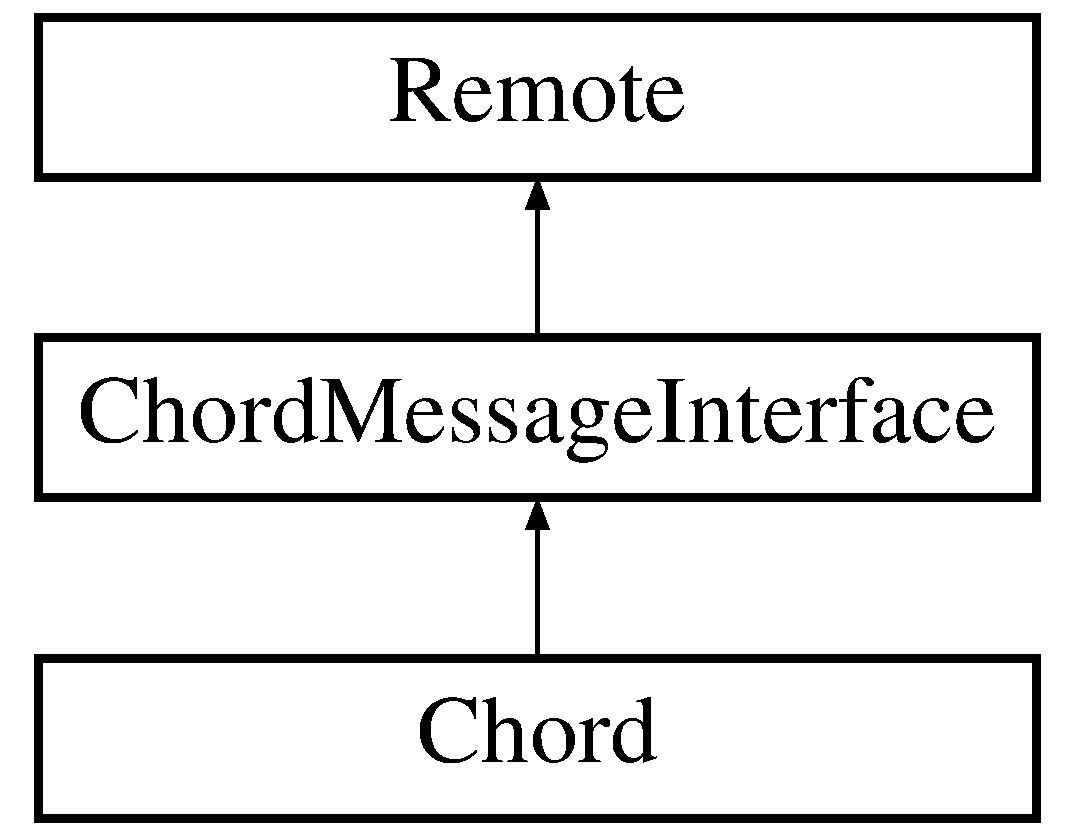
\includegraphics[height=3.000000cm]{interface_chord_message_interface}
\end{center}
\end{figure}
\subsection*{Public Member Functions}
\begin{DoxyCompactItemize}
\item 
\hyperlink{interface_chord_message_interface}{Chord\+Message\+Interface} \hyperlink{interface_chord_message_interface_ab07c08ba6088ef880eaf4ebae8281c51}{get\+Predecessor} ()  throws Remote\+Exception
\item 
\hyperlink{interface_chord_message_interface}{Chord\+Message\+Interface} \hyperlink{interface_chord_message_interface_a4e299d4b05537a4a07965dfe9f261fd0}{locate\+Successor} (int key)  throws Remote\+Exception
\item 
\hyperlink{interface_chord_message_interface}{Chord\+Message\+Interface} \hyperlink{interface_chord_message_interface_a7f47e9d5144a2af6904135bc05dfe8fd}{closest\+Preceding\+Node} (int key)  throws Remote\+Exception
\item 
void \hyperlink{interface_chord_message_interface_abc5a9483416a6b8ae7330b324869e236}{join\+Ring} (String Ip, int port)  throws Remote\+Exception
\item 
void \hyperlink{interface_chord_message_interface_abbb77f94541073d79284d35f970e0eb4}{notify} (\hyperlink{interface_chord_message_interface}{Chord\+Message\+Interface} j)  throws Remote\+Exception
\item 
boolean \hyperlink{interface_chord_message_interface_a8165b3fb53905e657c70b66223197561}{is\+Alive} ()  throws Remote\+Exception
\item 
int \hyperlink{interface_chord_message_interface_acead95d9a7196f05b656462ab78138eb}{get\+Id} ()  throws Remote\+Exception
\item 
void \hyperlink{interface_chord_message_interface_a59a01f2e913b6b2e4b60ba0b77c90eba}{put} (int guid, Input\+Stream file)  throws I\+O\+Exception, Remote\+Exception
\item 
Input\+Stream \hyperlink{interface_chord_message_interface_a4cdb461c48fe643f4fb5fa420d017eb3}{get} (int id)  throws I\+O\+Exception, Remote\+Exception
\item 
void \hyperlink{interface_chord_message_interface_ab4d46beae8cea347c827b5618ea16104}{delete} (int id)  throws I\+O\+Exception, Remote\+Exception
\end{DoxyCompactItemize}


\subsection{Member Function Documentation}
\index{Chord\+Message\+Interface@{Chord\+Message\+Interface}!closest\+Preceding\+Node@{closest\+Preceding\+Node}}
\index{closest\+Preceding\+Node@{closest\+Preceding\+Node}!Chord\+Message\+Interface@{Chord\+Message\+Interface}}
\subsubsection[{\texorpdfstring{closest\+Preceding\+Node(int key)}{closestPrecedingNode(int key)}}]{\setlength{\rightskip}{0pt plus 5cm}{\bf Chord\+Message\+Interface} Chord\+Message\+Interface.\+closest\+Preceding\+Node (
\begin{DoxyParamCaption}
\item[{int}]{key}
\end{DoxyParamCaption}
) throws Remote\+Exception}\hypertarget{interface_chord_message_interface_a7f47e9d5144a2af6904135bc05dfe8fd}{}\label{interface_chord_message_interface_a7f47e9d5144a2af6904135bc05dfe8fd}


Implemented in \hyperlink{class_chord_a77a9443c945cf5482f59edf685c1dc70}{Chord}.

\index{Chord\+Message\+Interface@{Chord\+Message\+Interface}!delete@{delete}}
\index{delete@{delete}!Chord\+Message\+Interface@{Chord\+Message\+Interface}}
\subsubsection[{\texorpdfstring{delete(int id)}{delete(int id)}}]{\setlength{\rightskip}{0pt plus 5cm}void Chord\+Message\+Interface.\+delete (
\begin{DoxyParamCaption}
\item[{int}]{id}
\end{DoxyParamCaption}
) throws I\+O\+Exception, Remote\+Exception}\hypertarget{interface_chord_message_interface_ab4d46beae8cea347c827b5618ea16104}{}\label{interface_chord_message_interface_ab4d46beae8cea347c827b5618ea16104}


Implemented in \hyperlink{class_chord_ab16ffb81226d722399a46d1acfd70e60}{Chord}.

\index{Chord\+Message\+Interface@{Chord\+Message\+Interface}!get@{get}}
\index{get@{get}!Chord\+Message\+Interface@{Chord\+Message\+Interface}}
\subsubsection[{\texorpdfstring{get(int id)}{get(int id)}}]{\setlength{\rightskip}{0pt plus 5cm}Input\+Stream Chord\+Message\+Interface.\+get (
\begin{DoxyParamCaption}
\item[{int}]{id}
\end{DoxyParamCaption}
) throws I\+O\+Exception, Remote\+Exception}\hypertarget{interface_chord_message_interface_a4cdb461c48fe643f4fb5fa420d017eb3}{}\label{interface_chord_message_interface_a4cdb461c48fe643f4fb5fa420d017eb3}


Implemented in \hyperlink{class_chord_a6fa6e161d33e337f53cc0f3e38e1791b}{Chord}.

\index{Chord\+Message\+Interface@{Chord\+Message\+Interface}!get\+Id@{get\+Id}}
\index{get\+Id@{get\+Id}!Chord\+Message\+Interface@{Chord\+Message\+Interface}}
\subsubsection[{\texorpdfstring{get\+Id()}{getId()}}]{\setlength{\rightskip}{0pt plus 5cm}int Chord\+Message\+Interface.\+get\+Id (
\begin{DoxyParamCaption}
{}
\end{DoxyParamCaption}
) throws Remote\+Exception}\hypertarget{interface_chord_message_interface_acead95d9a7196f05b656462ab78138eb}{}\label{interface_chord_message_interface_acead95d9a7196f05b656462ab78138eb}


Implemented in \hyperlink{class_chord_a7c6a50aff653bafc040f923c93061bdb}{Chord}.

\index{Chord\+Message\+Interface@{Chord\+Message\+Interface}!get\+Predecessor@{get\+Predecessor}}
\index{get\+Predecessor@{get\+Predecessor}!Chord\+Message\+Interface@{Chord\+Message\+Interface}}
\subsubsection[{\texorpdfstring{get\+Predecessor()}{getPredecessor()}}]{\setlength{\rightskip}{0pt plus 5cm}{\bf Chord\+Message\+Interface} Chord\+Message\+Interface.\+get\+Predecessor (
\begin{DoxyParamCaption}
{}
\end{DoxyParamCaption}
) throws Remote\+Exception}\hypertarget{interface_chord_message_interface_ab07c08ba6088ef880eaf4ebae8281c51}{}\label{interface_chord_message_interface_ab07c08ba6088ef880eaf4ebae8281c51}


Implemented in \hyperlink{class_chord_a3f1aadce3820e808c80662bb61a58e34}{Chord}.

\index{Chord\+Message\+Interface@{Chord\+Message\+Interface}!is\+Alive@{is\+Alive}}
\index{is\+Alive@{is\+Alive}!Chord\+Message\+Interface@{Chord\+Message\+Interface}}
\subsubsection[{\texorpdfstring{is\+Alive()}{isAlive()}}]{\setlength{\rightskip}{0pt plus 5cm}boolean Chord\+Message\+Interface.\+is\+Alive (
\begin{DoxyParamCaption}
{}
\end{DoxyParamCaption}
) throws Remote\+Exception}\hypertarget{interface_chord_message_interface_a8165b3fb53905e657c70b66223197561}{}\label{interface_chord_message_interface_a8165b3fb53905e657c70b66223197561}


Implemented in \hyperlink{class_chord_a0a677ced19cc0cb5afd2a695977aeb95}{Chord}.

\index{Chord\+Message\+Interface@{Chord\+Message\+Interface}!join\+Ring@{join\+Ring}}
\index{join\+Ring@{join\+Ring}!Chord\+Message\+Interface@{Chord\+Message\+Interface}}
\subsubsection[{\texorpdfstring{join\+Ring(\+String Ip, int port)}{joinRing(String Ip, int port)}}]{\setlength{\rightskip}{0pt plus 5cm}void Chord\+Message\+Interface.\+join\+Ring (
\begin{DoxyParamCaption}
\item[{String}]{Ip, }
\item[{int}]{port}
\end{DoxyParamCaption}
) throws Remote\+Exception}\hypertarget{interface_chord_message_interface_abc5a9483416a6b8ae7330b324869e236}{}\label{interface_chord_message_interface_abc5a9483416a6b8ae7330b324869e236}


Implemented in \hyperlink{class_chord_ace0b8d2768590d7527af155c6573cae7}{Chord}.

\index{Chord\+Message\+Interface@{Chord\+Message\+Interface}!locate\+Successor@{locate\+Successor}}
\index{locate\+Successor@{locate\+Successor}!Chord\+Message\+Interface@{Chord\+Message\+Interface}}
\subsubsection[{\texorpdfstring{locate\+Successor(int key)}{locateSuccessor(int key)}}]{\setlength{\rightskip}{0pt plus 5cm}{\bf Chord\+Message\+Interface} Chord\+Message\+Interface.\+locate\+Successor (
\begin{DoxyParamCaption}
\item[{int}]{key}
\end{DoxyParamCaption}
) throws Remote\+Exception}\hypertarget{interface_chord_message_interface_a4e299d4b05537a4a07965dfe9f261fd0}{}\label{interface_chord_message_interface_a4e299d4b05537a4a07965dfe9f261fd0}


Implemented in \hyperlink{class_chord_aa53f4f7c97122395a33d064460538db0}{Chord}.

\index{Chord\+Message\+Interface@{Chord\+Message\+Interface}!notify@{notify}}
\index{notify@{notify}!Chord\+Message\+Interface@{Chord\+Message\+Interface}}
\subsubsection[{\texorpdfstring{notify(\+Chord\+Message\+Interface j)}{notify(ChordMessageInterface j)}}]{\setlength{\rightskip}{0pt plus 5cm}void Chord\+Message\+Interface.\+notify (
\begin{DoxyParamCaption}
\item[{{\bf Chord\+Message\+Interface}}]{j}
\end{DoxyParamCaption}
) throws Remote\+Exception}\hypertarget{interface_chord_message_interface_abbb77f94541073d79284d35f970e0eb4}{}\label{interface_chord_message_interface_abbb77f94541073d79284d35f970e0eb4}


Implemented in \hyperlink{class_chord_a4de8b8464782dd96d88deeb35b2f27a2}{Chord}.

\index{Chord\+Message\+Interface@{Chord\+Message\+Interface}!put@{put}}
\index{put@{put}!Chord\+Message\+Interface@{Chord\+Message\+Interface}}
\subsubsection[{\texorpdfstring{put(int guid, Input\+Stream file)}{put(int guid, InputStream file)}}]{\setlength{\rightskip}{0pt plus 5cm}void Chord\+Message\+Interface.\+put (
\begin{DoxyParamCaption}
\item[{int}]{guid, }
\item[{Input\+Stream}]{file}
\end{DoxyParamCaption}
) throws I\+O\+Exception, Remote\+Exception}\hypertarget{interface_chord_message_interface_a59a01f2e913b6b2e4b60ba0b77c90eba}{}\label{interface_chord_message_interface_a59a01f2e913b6b2e4b60ba0b77c90eba}


Implemented in \hyperlink{class_chord_a1133387e1312ead8daf5c94c11ff3b78}{Chord}.



The documentation for this interface was generated from the following file\+:\begin{DoxyCompactItemize}
\item 
\hyperlink{_chord_message_interface_8java}{Chord\+Message\+Interface.\+java}\end{DoxyCompactItemize}

\hypertarget{class_chord_user}{}\section{Chord\+User Class Reference}
\label{class_chord_user}\index{Chord\+User@{Chord\+User}}
\subsection*{Public Member Functions}
\begin{DoxyCompactItemize}
\item 
\hyperlink{class_chord_user_ae885d3267350f3834158e42344854750}{Chord\+User} (int p)
\end{DoxyCompactItemize}
\subsection*{Static Public Member Functions}
\begin{DoxyCompactItemize}
\item 
static void \hyperlink{class_chord_user_a737455bbcfdae9ff4427063d77fb9038}{main} (String args\mbox{[}$\,$\mbox{]})  throws No\+Such\+Algorithm\+Exception 
\end{DoxyCompactItemize}


\subsection{Constructor \& Destructor Documentation}
\index{Chord\+User@{Chord\+User}!Chord\+User@{Chord\+User}}
\index{Chord\+User@{Chord\+User}!Chord\+User@{Chord\+User}}
\subsubsection[{\texorpdfstring{Chord\+User(int p)}{ChordUser(int p)}}]{\setlength{\rightskip}{0pt plus 5cm}Chord\+User.\+Chord\+User (
\begin{DoxyParamCaption}
\item[{int}]{p}
\end{DoxyParamCaption}
)}\hypertarget{class_chord_user_ae885d3267350f3834158e42344854750}{}\label{class_chord_user_ae885d3267350f3834158e42344854750}


\subsection{Member Function Documentation}
\index{Chord\+User@{Chord\+User}!main@{main}}
\index{main@{main}!Chord\+User@{Chord\+User}}
\subsubsection[{\texorpdfstring{main(\+String args[])}{main(String args[])}}]{\setlength{\rightskip}{0pt plus 5cm}static void Chord\+User.\+main (
\begin{DoxyParamCaption}
\item[{String}]{args\mbox{[}$\,$\mbox{]}}
\end{DoxyParamCaption}
) throws No\+Such\+Algorithm\+Exception\hspace{0.3cm}{\ttfamily [static]}}\hypertarget{class_chord_user_a737455bbcfdae9ff4427063d77fb9038}{}\label{class_chord_user_a737455bbcfdae9ff4427063d77fb9038}


The documentation for this class was generated from the following file\+:\begin{DoxyCompactItemize}
\item 
\hyperlink{_chord_user_8java}{Chord\+User.\+java}\end{DoxyCompactItemize}

\hypertarget{class_file_stream}{}\section{File\+Stream Class Reference}
\label{class_file_stream}\index{File\+Stream@{File\+Stream}}
Inheritance diagram for File\+Stream\+:\begin{figure}[H]
\begin{center}
\leavevmode
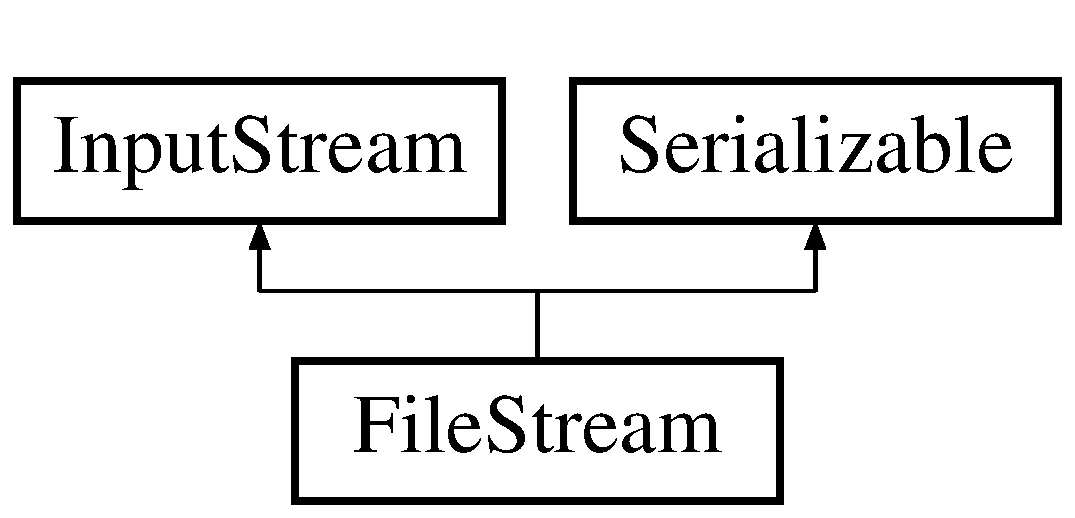
\includegraphics[height=2.000000cm]{class_file_stream}
\end{center}
\end{figure}
\subsection*{Public Member Functions}
\begin{DoxyCompactItemize}
\item 
\hyperlink{class_file_stream_a120b1fd6e4c74e93199d063da1c65b98}{File\+Stream} (String path\+Name)  throws File\+Not\+Found\+Exception, I\+O\+Exception 
\item 
\hyperlink{class_file_stream_aa919eed4082491d09520911563d44efd}{File\+Stream} ()  throws File\+Not\+Found\+Exception 
\item 
int \hyperlink{class_file_stream_a7f2ea40eff2241931a4ca971364cd532}{read} ()  throws I\+O\+Exception 
\item 
int \hyperlink{class_file_stream_a7dd240b96afa9e37f9a6bd8e4b99e48b}{available} ()  throws I\+O\+Exception 
\end{DoxyCompactItemize}


\subsection{Constructor \& Destructor Documentation}
\index{File\+Stream@{File\+Stream}!File\+Stream@{File\+Stream}}
\index{File\+Stream@{File\+Stream}!File\+Stream@{File\+Stream}}
\subsubsection[{\texorpdfstring{File\+Stream(\+String path\+Name)}{FileStream(String pathName)}}]{\setlength{\rightskip}{0pt plus 5cm}File\+Stream.\+File\+Stream (
\begin{DoxyParamCaption}
\item[{String}]{path\+Name}
\end{DoxyParamCaption}
) throws File\+Not\+Found\+Exception, I\+O\+Exception}\hypertarget{class_file_stream_a120b1fd6e4c74e93199d063da1c65b98}{}\label{class_file_stream_a120b1fd6e4c74e93199d063da1c65b98}
\index{File\+Stream@{File\+Stream}!File\+Stream@{File\+Stream}}
\index{File\+Stream@{File\+Stream}!File\+Stream@{File\+Stream}}
\subsubsection[{\texorpdfstring{File\+Stream()}{FileStream()}}]{\setlength{\rightskip}{0pt plus 5cm}File\+Stream.\+File\+Stream (
\begin{DoxyParamCaption}
{}
\end{DoxyParamCaption}
) throws File\+Not\+Found\+Exception}\hypertarget{class_file_stream_aa919eed4082491d09520911563d44efd}{}\label{class_file_stream_aa919eed4082491d09520911563d44efd}


\subsection{Member Function Documentation}
\index{File\+Stream@{File\+Stream}!available@{available}}
\index{available@{available}!File\+Stream@{File\+Stream}}
\subsubsection[{\texorpdfstring{available()}{available()}}]{\setlength{\rightskip}{0pt plus 5cm}int File\+Stream.\+available (
\begin{DoxyParamCaption}
{}
\end{DoxyParamCaption}
) throws I\+O\+Exception}\hypertarget{class_file_stream_a7dd240b96afa9e37f9a6bd8e4b99e48b}{}\label{class_file_stream_a7dd240b96afa9e37f9a6bd8e4b99e48b}
\index{File\+Stream@{File\+Stream}!read@{read}}
\index{read@{read}!File\+Stream@{File\+Stream}}
\subsubsection[{\texorpdfstring{read()}{read()}}]{\setlength{\rightskip}{0pt plus 5cm}int File\+Stream.\+read (
\begin{DoxyParamCaption}
{}
\end{DoxyParamCaption}
) throws I\+O\+Exception}\hypertarget{class_file_stream_a7f2ea40eff2241931a4ca971364cd532}{}\label{class_file_stream_a7f2ea40eff2241931a4ca971364cd532}


The documentation for this class was generated from the following file\+:\begin{DoxyCompactItemize}
\item 
\hyperlink{_file_stream_8java}{File\+Stream.\+java}\end{DoxyCompactItemize}

\chapter{File Documentation}
\hypertarget{_chord_8java}{}\section{Chord.\+java File Reference}
\label{_chord_8java}\index{Chord.\+java@{Chord.\+java}}
\subsection*{Classes}
\begin{DoxyCompactItemize}
\item 
class \hyperlink{class_chord}{Chord}
\end{DoxyCompactItemize}

\hypertarget{_chord_message_interface_8java}{}\section{Chord\+Message\+Interface.\+java File Reference}
\label{_chord_message_interface_8java}\index{Chord\+Message\+Interface.\+java@{Chord\+Message\+Interface.\+java}}
\subsection*{Classes}
\begin{DoxyCompactItemize}
\item 
interface \hyperlink{interface_chord_message_interface}{Chord\+Message\+Interface}
\end{DoxyCompactItemize}

\hypertarget{_chord_user_8java}{}\section{Chord\+User.\+java File Reference}
\label{_chord_user_8java}\index{Chord\+User.\+java@{Chord\+User.\+java}}
\subsection*{Classes}
\begin{DoxyCompactItemize}
\item 
class \hyperlink{class_chord_user}{Chord\+User}
\end{DoxyCompactItemize}

\hypertarget{_file_stream_8java}{}\section{File\+Stream.\+java File Reference}
\label{_file_stream_8java}\index{File\+Stream.\+java@{File\+Stream.\+java}}
\subsection*{Classes}
\begin{DoxyCompactItemize}
\item 
class \hyperlink{class_file_stream}{File\+Stream}
\end{DoxyCompactItemize}

\hypertarget{_r_e_a_d_m_e_8md}{}\section{R\+E\+A\+D\+M\+E.\+md File Reference}
\label{_r_e_a_d_m_e_8md}\index{R\+E\+A\+D\+M\+E.\+md@{R\+E\+A\+D\+M\+E.\+md}}

%--- End generated contents ---

% Index
\backmatter
\newpage
\phantomsection
\clearemptydoublepage
\addcontentsline{toc}{chapter}{Index}
\printindex

\end{document}
